%%4 Project approach 
\section{Project Approach}
\label{sec:projectapproach}
%Give a high-level description of your envisioned solution to the problem. Substantiate any relevant choices in terms of design & technology. 

In this section, we outline the key decisions outlined in designing our application. The detailed aspects of our software architecture, technology choices, and design choices will be further discussed. This was an integral step in the initial planning on the project and was still re-visited throughout the project given the architectural complexity and novelty of the technologies used.

\subsection{Software Architecture}

\subsection{Technology Choices}

\indent \indent With the exception of AWS SageMaker and AWS Translate, the client is very lenient with which of the Amazon services we use. AWS SageMaker plays an important role in our application for developing our translation service using machine learning. It provides a platform to easily apply ML models and is scalable in the building and training process, offering efficiency and cost optimization. With the current knowledge of the group, Figure \ref{fig:Services} shows our current approach to the project's development though many of these services may change. This is due to our weekly meetings with the client and discussions regarding our progress as well as consulting them in case we need assistance with any of their services. While our exact methodology will be addressed in Section \ref{sec:developmentmethodology}, the client has explicitly stated that our approach should allow for feedback and opinions (from the client and development team) and maintainability such that we can have a \textit{flexible} approach. This flexibility means we can re-evaluate and deviate from the original project plan throughout development and perhaps use alternative services or implementations. 

\indent Flexibility in mind, our high-level approach and requirements were stagnant. There is a plethora of AWS services we can use so as a result, In the initial stages of the project, we intend to familiarize ourselves with the AWS platform and some of its various services to integrate them into our development and enhance our understanding of the project as well as the client's requests. Once familiarized with the AWS ecosystem,through research and use of these services, we felt more comfortable beginning the implementation process.

\indent In developing the implementation our initial plan was to start building the application in the shape of a working Front-end, Back-end, and communication between the two. Then, we intend to directly cover the functional requirements presented in Section \ref{sec:Requirements} in order of importance, while still keeping non-functional requirements in mind.


%%UPDATED DIAGRAM:
\begin{figure}[ht]
    \centering
    \begin{tikzpicture}[
  block/.style={rectangle, draw, text width=2.5cm, align=center, minimum height=2em},
  arrow/.style={->, thick},
  text_below/.style={align=center, text width=3cm}
]
  \node[block] (building) {Building and Shipping};
  \node[block, below= 2cm of building] (gateway) {Gateway \&\\ Communication};
  \node[block, left = 1.1cm of gateway] (frontend) {Front End};
  \node[block, right = 1.1cm of gateway] (backend) {Back End};
  \node[block, right= 1.1cm and of backend] (ml) {ML pipeline};
  \node[block, above = 1.0 cm of ml] (data) {Database};
  

  \node[text_below, right=0.1cm of building] {AWS Amplify \\ AWS CDK};
  \node[text_below, below=0.1cm of frontend] {AWS Amplify\\Studio};
  \node[text_below, below=0.1cm of gateway] {AWS Chalice \\ AWS AppSync};
  \node[text_below, below=0.1cm of backend] {AWS Amplify};
  \node[text_below, below=0.1cm of ml] {AWS Sagemaker \&\\ Amazon Translate};
  \node[text_below, above=0.1cm of data] {DynamoDB};

  \draw[arrow] (building) -- (frontend);
  \draw[arrow] (building) -- (gateway);
  \draw[arrow] (building) -- (backend);
  \draw[arrow] (backend) -- (ml);
  \draw[arrow] (frontend) -- (gateway);
  \draw[arrow] (gateway) -- (backend);
  \draw[arrow] (backend) -- (data);
  
\end{tikzpicture}
    \caption{Use of AWS services in development}
    \label{fig:Services}
\end{figure}

\subsection{Design Choices}

\indent Figure \ref{fig:rough_sketch} presents the \acrshort{ui} the group has envisioned for the project. We intend for the application to roughly follow this design where we see the original text on the left and translated side on the right. We also intend to give the user the ability to easily translate a different blog post (URL), change the translation language (Language), and the method of translation (Translation). As part of our design, we intend for translations and objects to appear side by side, providing a clear alignment between the original and translated blog.

\indent This initial design is predominantly a product of the client's exact wishes. Claiming that they wanted these exact features visually displayed on the web application. That said, it still follows common design heuristics which are significant to build a bridge between the user and the application to achieve a certain goal \cite{DesignHeuristic}. The design is simplistic, efficient, and the user's has been taken into account, meaning the UI/UX allows for usability of the application on the basis of the user's needs while prioritizing user satisfaction through this feedback cycle \cite{DesignHeuristic}. The accessibility of the application is another important aspect since users with disabilities should be able to use the application as easily as any other user, meaning the final product will follow general \href{https://www.w3.org/TR/WCAG21/}{WCAG2.1} guidelines. 

%%Image of Project Plan
\begin{figure}[ht]
    \centering
    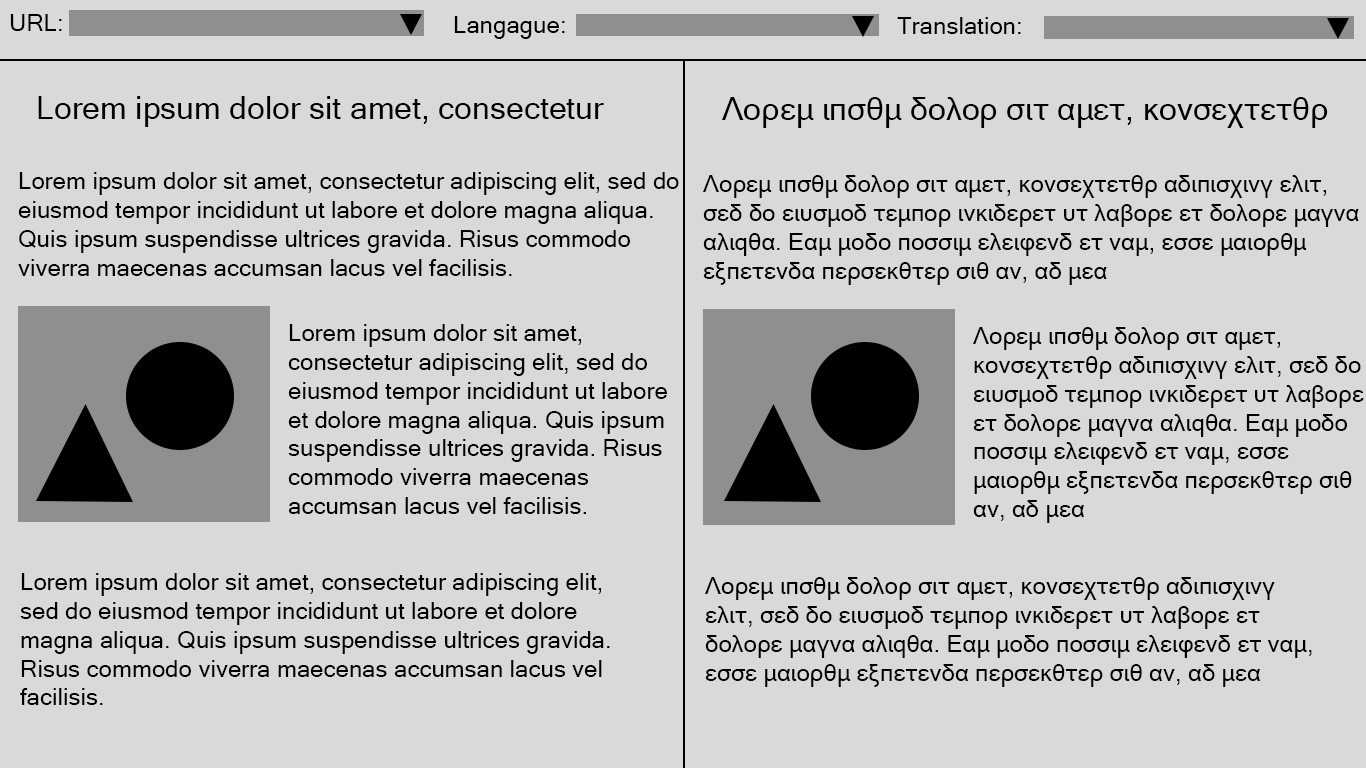
\includegraphics[width=0.8\textwidth]{images/AWS_Blog_translate_rough_sketch.png}
    \caption{Visual Design of Application}
    \label{fig:rough_sketch}
\end{figure}